\exercisesheader{}

% 15 - air_quality_shortened

\eoce{\qt{Air quality\label{air_quality_shortened}}
Air quality measurements were collected in 
a random sample of 25 country capitals in 2013, and then again in the same 
cities in 2014. We would like to use these data to compare
average air quality between the two years.
Should we use a paired or non-paired test? Explain your reasoning.
}{}

% 16 - tf_paired

\eoce{\qt{True / False: paired\label{tf_paired}} Determine if the following 
statements are true or false. If false, explain.
\begin{parts}
\item In a paired analysis we first take the difference of each pair of observations, 
and then we do inference on these differences.
\item Two data sets of different sizes cannot be analyzed as paired data.
\item Consider two sets of data that are paired with each other.
Each observation in one data set has a natural correspondence with 
exactly one observation from the other data set.
\item Consider two sets of data that are paired with each other.
Each observation in one data set is subtracted from the average of the 
other data set's observations.
\end{parts}
}{}

% 17 - paired_or_not_1

\eoce{\qt{Paired or not? Part I\label{paired_or_not_1}} In each of the following 
scenarios, determine if the data are paired.
\begin{parts}
\item Compare pre- (beginning of semester) and post-test (end of semester) 
scores of students.
\item Assess gender-related salary gap by comparing salaries of randomly 
sampled men and women.
\item Compare artery thicknesses at the beginning of a study and after 2 years 
of taking Vitamin E for the same group of patients.
\item Assess effectiveness of a diet regimen by comparing the before and after 
weights of subjects.
\end{parts}
}{}

% 18 - paired_or_not_2

\eoce{\qt{Paired or not? Part II\label{paired_or_not_2}} In each of the following 
scenarios, determine if the data are paired.
\begin{parts}
\item We would like to know if Intel's stock and Southwest Airlines' stock have 
similar rates of return. To find out, we take a random sample of 50 days, and 
record Intel's and Southwest's stock on those same days.
\item We randomly sample 50 items from Target stores and note the price for 
each. Then we visit Walmart and collect the price for each of those same 50 
items.
\item A school board would like to determine whether there is a difference in 
average SAT scores for students at one high school versus another high school 
in the district. To check, they take a simple random sample of 100 students 
from each high school.
\end{parts}
}{}

% 19 - global_warming_v2_1

\eoce{\qt{Global warming, Part I\label{global_warming_v2_1}}
Let's consider a limited set of climate data,
examining temperature differences in 1948 vs~2018.
We sampled 197 locations from the
National Oceanic and Atmospheric Administration's
(NOAA) historical data,
where the data was available for both years of interest.
We want to know: were there more days with temperatures
exceeding 90\textdegree{}F in 2018 or
in~1948?\footfullcite{webpage:noaa_1948_2018}
The difference in number of days exceeding 90\textdegree{}F
(number of days in 2018 - number of days in 1948) was calculated
for each of the 197 locations.
The average of these differences was 2.9 days with 
a standard deviation of 17.2 days.
We are interested in determining whether these data provide
strong evidence that there were more days in 2018 that
exceeded 90\textdegree{}F from NOAA's weather
stations.\vspace{3mm}

\noindent%
\begin{minipage}[c]{0.65\textwidth}
\begin{parts}
\item
    Is there a relationship between the observations collected
    in 1948 and 2018?
    Or are the observations in the two groups independent?
    Explain.
\item
    Write hypotheses for this research in symbols and in words.
\item
    Check the conditions required to complete this test.
    A histogram of the differences is given to the right.
\item
    Calculate the test statistic and find the p-value.
\item
    Use $\alpha = 0.05$ to evaluate the test,
    and interpret your conclusion in context.
\item
    What type of error might we have made?
    Explain in context what the error means.
\item
    Based on the results of this hypothesis test,
    would you expect a confidence interval for the
    average difference between the number of days
    exceeding 90\textdegree{}F from 1948 and 2018
    to include 0?
    Explain your reasoning.
\end{parts}
\end{minipage}
\begin{minipage}[c]{0.02\textwidth}
\ 
\end{minipage}
\begin{minipage}[c]{0.32\textwidth}
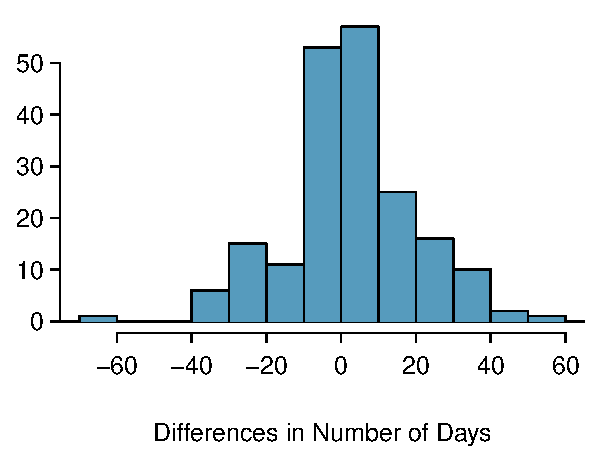
\includegraphics[width=\textwidth]{ch_inference_for_means/figures/eoce/global_warming_v2_1/global_warming_v2_1_diffs}
\end{minipage}
% library(openintro); d <- climate70$dx90_2018 - climate70$dx90_1948; mean(d); sd(d); length(d); t.test(d)
}{}

\D{\newpage}
% 20 - hs_beyond_1

\eoce{\qt{High School and Beyond, Part I\label{hs_beyond_1}} The National Center of 
Education Statistics conducted a survey of high school seniors, collecting test 
data on reading, writing, and several other subjects. Here we examine a simple 
random sample of 200 students from this survey. Side-by-side box plots of 
reading and writing scores as well as a histogram of the differences in scores 
are shown below.
\begin{center}
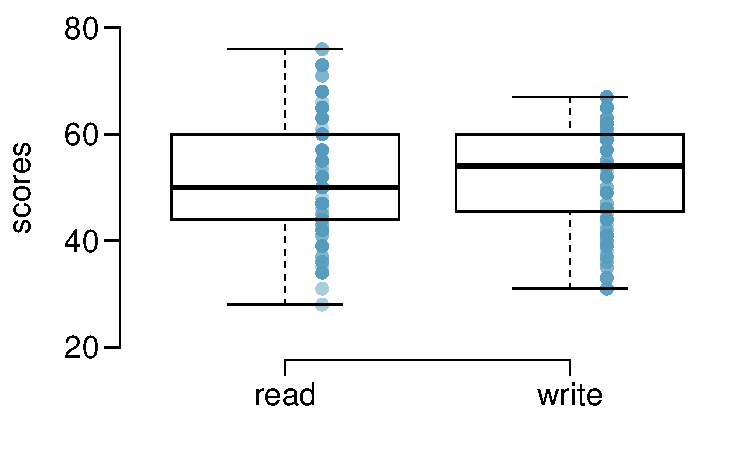
\includegraphics[width=0.44\textwidth]{ch_inference_for_means/figures/eoce/hs_beyond_1/hs_beyond_read_write_box.pdf}
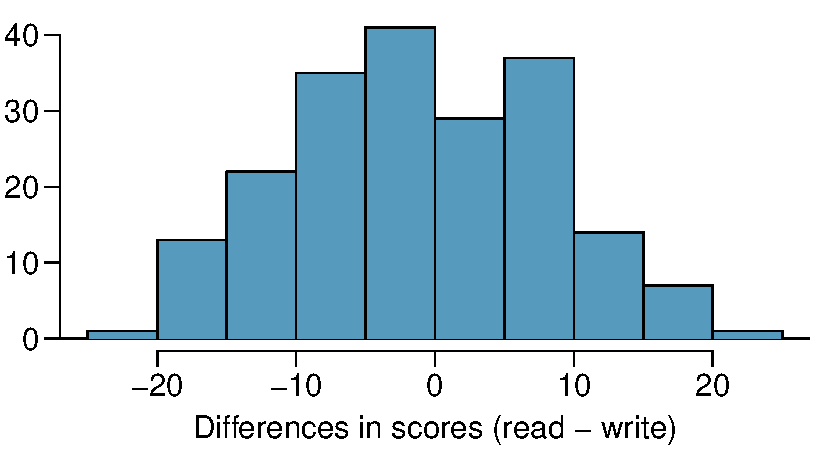
\includegraphics[width=0.54\textwidth]{ch_inference_for_means/figures/eoce/hs_beyond_1/hs_beyond_diff_hist.pdf}
\end{center}
\begin{parts}
\item Is there a clear difference in the average reading and writing scores?
\item Are the reading and writing scores of each student independent of each 
other?
\item Create hypotheses appropriate for the following research question: is 
there an evident difference in the average scores of students in the reading 
and writing exam?
% is there evidence that students on average perform differently on the reading and writing exam?
\item Check the conditions required to complete this test.
\item The average observed difference in scores is 
$\bar{x}_{read-write} = -0.545$, and the standard deviation of the differences 
is 8.887 points. Do these data provide convincing evidence of a difference 
between the average scores on the two exams?
\item What type of error might we have made? Explain what the error means in 
the context of the application.
\item Based on the results of this hypothesis test, would you expect a 
confidence interval for the average difference between the reading and writing 
scores to include 0? Explain your reasoning.
\end{parts}
}{}

% 21 - global_warming_v2_2

\eoce{\qt{Global warming, Part II\label{global_warming_v2_2}}
We considered the change in the number of days exceeding
90\textdegree{}F from 1948 and 2018 at 197 randomly sampled
locations from the NOAA database in
Exercise~\ref{global_warming_v2_1}.
The mean and standard deviation of the reported differences
are 2.9 days and 17.2 days.
\begin{parts}
\item
    Calculate a 90\% confidence interval for the average
    difference between number of days exceeding 90\textdegree{}F
    between 1948 and 2018.
    We've already checked the conditions for you.
\item
    Interpret the interval in context.
\item
    Does the confidence interval provide convincing evidence
    that there were more days exceeding 90\textdegree{}F
    in 2018 than in 1948 at NOAA stations?
    Explain.
\end{parts}
}{}

% 22 - hs_beyond_2

\eoce{\qt{High school and beyond, Part II\label{hs_beyond_2}} We considered the 
differences between the reading and writing scores of a random sample of 200 
students who took the High School and Beyond Survey in Exercise~\ref{hs_beyond_1}. The 
mean and standard deviation of the differences are 
$\bar{x}_{read-write} = -0.545$ and 8.887 points.
\begin{parts}
\item Calculate a 95\% confidence interval for the average difference between 
the reading and writing scores of all students.
\item Interpret this interval in context.
\item Does the confidence interval provide convincing evidence that there is a 
real difference in the average scores? Explain.
\end{parts}
}{}
